\section{O grupach krótko}

Grupa jaka jest każdy wie. Nas ostatecznie będą interesowały grupy zwarte i lokalnie zwarte. Najpierw ujednorodnijmy wiedzę z algebry.

\subsection{Grupy wolne}

Grupa wolna $F_S$ o generatorach $S$ to zbiór ciągów elementów z $S\cup S^{-1}$ gdzie jedyne skrócenia jakie akceptujemy to $ss^{-1}$ dla $s\in S$.

\begin{example}[m]
  \item Liczby całkowite $\Z$ tworzą grupę wolną o jednym generatorze.
  \item Grupę $F_2$ o generatorach $s$, $t$ można przedstawić jako nieskończone drzewo $4$-regularne. Wtedy elementy $F_2$ to ścieżki startujące w pewnym wyróżnionym wierzchołku.
    \begin{center}
      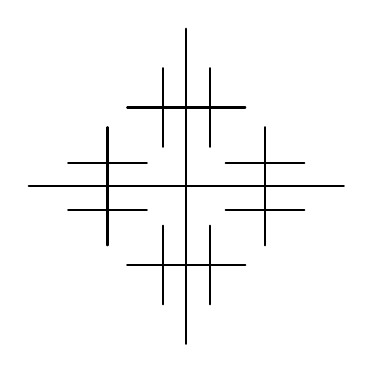
\begin{tikzpicture}[thick, cap=round]
        \draw (-2,0)--(2,0);
        \draw (0,-2)--(0,2);
        
        \draw (-1,-.75)--(-1,.75);
        \draw (1,-.75)--(1,.75);
        \draw (-.75,1)--(.75,1);
        \draw (-.75,-1)--(.75,-1);

        \draw (-1.5,.3)--(-.5,.3);
        \draw (-1.5,-.3)--(-.5,-.3);
        \draw (1.5,-.3)--(.5,-.3);
        \draw (1.5,.3)--(.5,.3);

        \draw (-.3, .5)--(-.3,1.5);
        \draw (.3, .5)--(.3,1.5);
        \draw (-.3, -.5)--(-.3,-1.5);
        \draw (.3, -.5)--(.3,-1.5);
      \end{tikzpicture}
    \end{center}
\end{example}

\begin{lemma}{}{}
  Każda grupa $G$ jest obrazem pewnej grupy wolnej $F_S$ dla pewnego zbioru generatorów $S$.
\end{lemma}

\begin{definition}{prezentacja grupy}{}
  Niech $S$ będzie zbiorem generatorów z lematu wyżej, a $R$ - jądrem homomorfizmu $G\to F_S$. Wtedy $\langle S|R\rangle$ nazywamy \textbf{prezentacją grupy $G$}, gdzie $S$ to jej generatory, a $R$ - relacje.
\end{definition}

\begin{example}
Grupa $S_3$ permutacji zbioru trzyelemntowego ma prezentację 
$$\langle \sigma_1, \sigma_2|\sigma_1^2=\sigma_2^1=(\sigma_1\sigma_2)^3=id\rangle,$$ 
gdzie $\sigma_i$ to permutacja $(i, i+1)$.
\end{example}

Powstaje pytanie jak sprawdzać, czy dana podgrupa $H\leq G$ jest wolna. Na przykład czy podgrupa
$$H=\left\langle\begin{bmatrix}1&2\\0&1\end{bmatrix},\begin{bmatrix}1&0\\2&1\end{bmatrix}\right\rangle\leq SL_2(\R)$$ 
generują podgrupę wolną. Z pomocą przychodzi lemat o ping pongu, który w najprostszej wersji mówi:

\begin{lemma}{ping pong}{}
  Niech $a, b\in G$ będą elementami grupy działającej na pewnym zbiorze $X$. Jeśli istnieją niepuste, rozłączne podzbiory $A,B\subseteq X$ takie, że dla wszystkich $n\in \N$ $a^nB\subseteq A$ oraz $b^nA\subseteq B$ to podgrupa $\langle a,b\rangle$ jest wolna.
\end{lemma}

\begin{proof}
  Weźmy dowolne słowo $w=a^{n_k}b^{m_k}...a^{n_1}b^{m_1}$ w skróconej postaci. 

  Na początek załóżmy, że $n_1$ oraz $n_k$ nie są zerowe oraz $m_k=0$. Wtedy dla $x\in B$ gramy w ping ponga idąc od końca słowa $w$. $a^{n_k}x\in A$, więc $b^{n_{k-1}}(a^{n_k}x)\in B$ i tak dalej aż dochodzimy do $b^{m_1}...a^{n_k}x\in B$, które $a^{n_1}$ wrzuca z powrotem w $A$. Ponieważ $A\cap B=\emptyset$ to $A\ni wx\neq x\in B$, czyli $w\neq 1$. 

  Pozostaje nam rozważyć przypadek, kiedy słowo zaczyna się literką $a$ i kończy literką $b$, czyli jest postaci $w=a^n w'b^m$. Załóżmy nie wprost, że $a^nw'b^m=1$, wtedy $a^n(a^nw'b^m)a^{-n}=a^n1a^{-n}=1$, ale $a^{2n}w'b^ma^{-n}$ jest słowem zaczynającym i kończącym się potęgą litery $a$ - dostajemy sprzeczność z rozumowaniem wyżej.
\end{proof}

Ćwiczenie dla studenta: jak uogólnić powyższy lemat by sprawdzać, czy $\langle a_1,...,a_n\rangle\leq G$ jest grupą wolną?

\subsection{Graf Cayley'a}

\begin{definition}{graf Cayley}{}
  Niech $G=\langle S|R\rangle$ będzie prezentacją grupy. Graf Cayley dla zbioru generatorów $S$ definiujemy jako skierowany graf $\Gamma(G, S)$ gdzie
  \begin{itemize}
    \item wierzchołki to elementy grupy $V=G$
    \item a krawędzie to przesunięcia o generator lub jego odwrotność, $E=\{(v,vs)\;:\;v\in G, s\in S\cup S^{-1}\}$.
  \end{itemize}
\end{definition}

Z racji że z każdego wierzchołka grafu Cayley wyprowadzamy po jednej krawędzi dla każdego generatora, to jest on zawsze $|S|$-regularny oraz spójny.

\begin{example}
  Rozważmy grupę $S_3=\langle \sigma_1, \sigma_2|\sigma_1^2=\sigma_2^2=(\sigma_1\sigma_2)^3\rangle$. Wtedy jej graf Cayley to 
  \begin{center}
    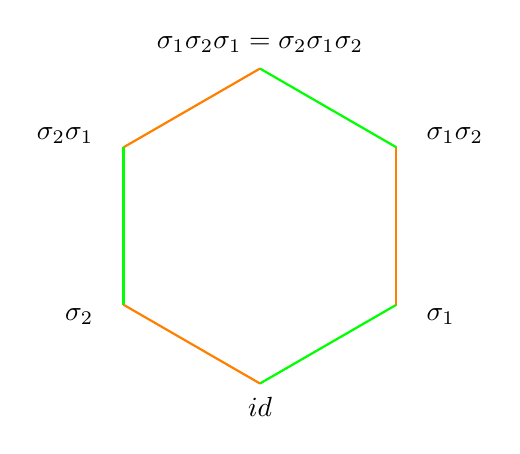
\begin{tikzpicture}
      \foreach \i in {0,2,4} {
        \draw[green, thick] ({-90+\i*60}:2)--({-90+(\i+1)*60}:2);
        \draw[orange, thick] ({-30+\i*60}:2)--({-30+(\i+1)*60}:2);
      }

      \node at (-90:2.3) {$id$};
      \node[anchor=west] at (-30:2.3) {$\sigma_1$};
      \node[anchor=west] at (30:2.3) {$\sigma_1\sigma_2$};
      \node at (90:2.3) {$\sigma_1\sigma_2\sigma_1=\sigma_2\sigma_1\sigma_2$};
      \node[anchor=east] at (150:2.3) {$\sigma_2\sigma_1$};
      \node[anchor=east] at (-150:2.3) {$\sigma_2$};
    \end{tikzpicture}
  \end{center}
  przy czym każdą krawędź rozumiemy jako parę strzałek -> $\sigma_i^{-1}=\sigma_i$.
\end{example}

% Dlaczego grafy Cayley są przydatne?
% \begin{enumerate}
%   \item Daje za darmo działanie grupy na pewnej przestrzeni (o ujemnej krzywiźnie) przez mnożenie z prawej strony.
%   \item Jest nawet lepiej, na grafie Cayley jesteśmy w stanie zdefiniować metrykę, interpretując każdą krawędź jako odcinek $[0,1]$. Wtedy grupa staje się przestrzenią metryczną/działającą na przestrzeni metrycznej.
%   % \item {\color{red}kwantowe pyśki i bity?? jakiś hamiltonian}
% \end{enumerate}

\subsection{Grupy topologiczne}

Bardzo często chcemy traktować grupę w ten sam sposób co każdą inna przestrzeń. Możemy oczywiście zapomnieć całkowicie o działaniach, które sprawiają że grupa jest grupą i definiować topologię tak jak nam się żywnie podoba. Możemy też być bardziej wybredni i wymagać od topologii, aby własności cechujące grupy były topologiczne.

\begin{definition}{}{}
  Grupa $G$ jest grupą topologiczną, jeśli potrafimy na niej zdefiniować topologię w taki sposób, aby funkcje
  \begin{itemize}
    \item mnożenia $\mu:G\times G\to G$, $\mu(g,h)=gh$
    \item oraz odwrotności $\iota:G\to G$, $\iota(g)=g^{-1}$
  \end{itemize}
  były ciągłe.
\end{definition}

\begin{example}[m]
\item Grupa $\Z$ z topologią dyskretną jest grupą topologiczną. Nawet lepiej - na każdej innej grupie również możemy zadać topologię dyskretną!
\item Torusik $T^1=S^1$ interpretowany jako zespolony okrąg jednostkowy, $\{e^{i\theta}\;:\;\theta\in[0,2\pi)\}$, jest grupą z topologią przychodzącą z odcinka $[0,2\pi)$.
\item Wszelakie grupy macierzy, czyli np. $SL(n)$, $SO(n)$, $SU(n)$ etc. Są to nawet \emph{grupy Liego} (mają strukturę różniczkowalną).
\end{example}

Bardzo przyjemnym rodzajem grup topologicznych są grupy zwarte. Jeśli oznaczymy przez $G_0$ otoczenie identyczności w zwartej grupie $G$, to potrafimy tym $G_0$ pokryć całą grupę przesuwając je przez elementy grupy. Ale grupa jest zwarta, więc wystarczy skończenie wiele przesunięć. To oznacza, że $G/G_0$ jest skończona.

Inną przyjemną własnością grup zwartych jest istnienie na nich miary niezmienniczej na przesunięcia, nazywanej \acc{miarą Haara}. Nie jest to jednak cecha wyłączna dla grup zwartych. Warunek zwartości można osłabić, nie tracąc przy tym istnienia miary Haara. Do kontemplowania miary Haara wrócimy w przyszłości.

\begin{definition}{przestrzeń lokalnie zwarta}{}
  Powiemy, że przestrzeń topologiczna $X$ jest \buff{lokalnie zwarta}, jeśli dla każdego punktu $x\in X$ potrafimy znaleźć otoczenie $x\in U\subseteq X$ takie, że $U$ jest przestrzenią zwartą.
\end{definition}

\begin{example}[m]
\item Bardzo przyjemną grupą zwartą (a więc i lokalnie zwartą) jest torus $S^1=T^1$.
\item Liczby rzeczywiste z dodawaniem, $(\R, +)$ nie są zwarte, ale są lokalnie zwarte.
\item Istnieją dokładnie trzy lokalnie zwarte ciała, których grupy jednostek są grupami lokalnie zwartymi:
  \begin{enumerate}
    \item $\R$, $\C$,
    \item ciała liczb $p$-adycznych, $Q_p$ gdzie liczby to kombinacje liniowe (niekoniecznie skończone) liczb $p^{k}$ dla $k\in\Z$,
    \item szeregi Lauranta o współczynnikach w ciele skończonym, $F_p((t))$.
  \end{enumerate}
\end{example}

% \section{Produkty tensorowe (wszelakiej maści)}
%
% Niech $V$ i $W$ będą przestrzeniami tensorowymi. Od dziecka wiemy jak zrobić ich sumę prostą, $V\oplus W$: rozważamy zbiór uporządkowanych par $(v,w)$ elementów $v\in V$ oraz $w\in W$ z operacją dodawania po współrzędnych $(v,w)+(v',w')=(v+v', w+w')$ oraz mnożeniem przez elementy ciała $r(v,w)=(rv,rw)$.


% \section{Wiązki wektorowe (i nie tylko)}
%









